\hypertarget{_s_c_p_i__input_buffer_8h}{\section{scpi/\-S\-C\-P\-I\-\_\-input\-Buffer.h File Reference}
\label{_s_c_p_i__input_buffer_8h}\index{scpi/\-S\-C\-P\-I\-\_\-input\-Buffer.\-h@{scpi/\-S\-C\-P\-I\-\_\-input\-Buffer.\-h}}
}
This graph shows which files directly or indirectly include this file\-:\nopagebreak
\begin{figure}[H]
\begin{center}
\leavevmode
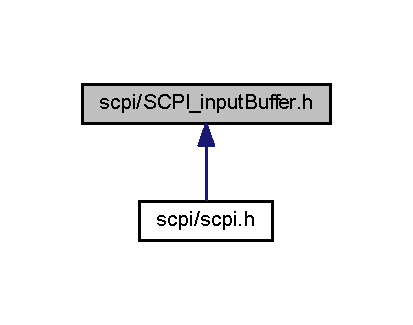
\includegraphics[width=198pt]{_s_c_p_i__input_buffer_8h__dep__incl}
\end{center}
\end{figure}


\subsection{Detailed Description}
This file provides the S\-C\-P\-I input buffer and the functions that are used to access and manage it

The input buffer stores D\-A\-Bs, G\-E\-T messages, and E\-N\-D messages. The input buffer then delivers these messages to the parser in the order that they were received from the I/\-O control.

This file should not need to be edited by the user 